% Graphical abstract (Elsevier: >= 531 x 1328 px (h x w), readable at 5 x 13 cm). Right panel after the final runs.
\documentclass[tikz,border=2pt]{standalone}
\usepackage{amsmath,amssymb}\usepackage{mathptmx}\usepackage{bm}
\usetikzlibrary{positioning,arrows.meta,calc}
\definecolor{cSo}{HTML}{1565C0}\definecolor{cAn}{HTML}{388E3C}\definecolor{cVei}{HTML}{F57C00}
\definecolor{cFn}{HTML}{7B1FA2}\definecolor{cPg}{HTML}{C62828}
\begin{document}
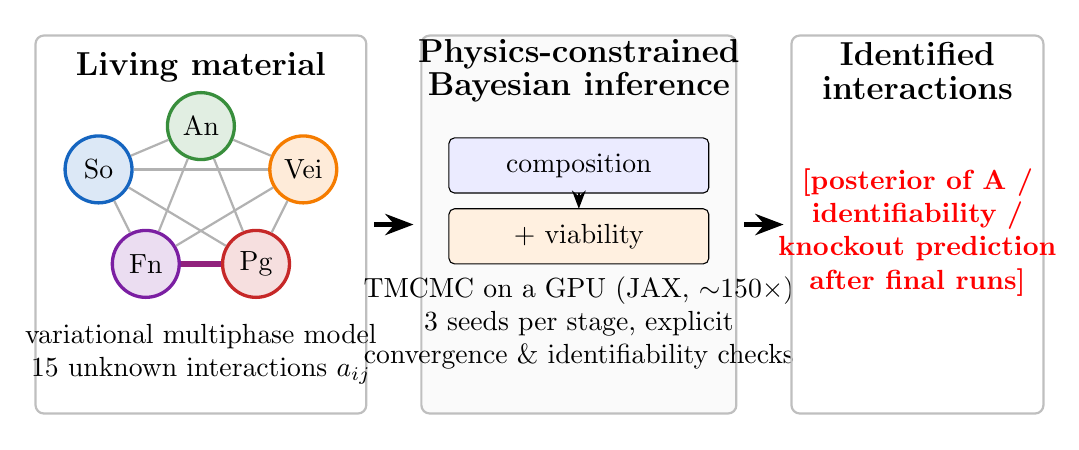
\begin{tikzpicture}[x=1cm,y=1cm,>=Stealth,font=\large,
  sp/.style={circle,draw=#1,fill=#1!15,very thick,minimum size=8.5mm,inner sep=0pt,font=\normalsize},
  panel/.style={draw=gray!50,rounded corners=3pt,thick}]
\useasboundingbox (0,0) rectangle (13,5);
% left: data + model
\draw[panel] (0.1,0.1) rectangle (4.3,4.9);
\node[font=\large\bfseries] at (2.2,4.5) {Living material};
\node[sp=cSo] (So) at (0.9,3.2) {So};
\node[sp=cAn] (An) at (2.2,3.75) {An};
\node[sp=cVei] (Vei) at (3.5,3.2) {Vei};
\node[sp=cFn] (Fn) at (1.5,2.0) {Fn};
\node[sp=cPg] (Pg) at (2.9,2.0) {Pg};
\foreach \a/\b in {So/An,So/Vei,An/Vei,So/Fn,An/Fn,Vei/Fn,So/Pg,An/Pg,Vei/Pg}{\draw[gray!60,thick] (\a)--(\b);}
\draw[cFn!70!cPg,line width=2.4pt] (Fn)--(Pg);
\node[align=center,font=\normalsize] at (2.2,0.85) {variational multiphase model\\ 15 unknown interactions $a_{ij}$};
% middle: inference
\draw[->,line width=1.6pt] (4.4,2.5)--(4.9,2.5);
\draw[panel,fill=gray!4] (5.0,0.1) rectangle (9.0,4.9);
\node[font=\large\bfseries,align=center] at (7.0,4.45) {Physics-constrained\\[-2pt] Bayesian inference};
\foreach \i/\t/\c in {0/composition/blue!8,1/{+ viability}/orange!12}{
  \node[draw,rounded corners=2pt,fill=\c,minimum width=3.3cm,minimum height=0.7cm,font=\normalsize] at (7.0,3.25-\i*0.9) {\t};}
\draw[->,thick] (7.0,2.9)--(7.0,2.7);
\node[align=center,font=\normalsize] at (7.0,1.25) {TMCMC on a GPU (JAX, $\sim$150$\times$)\\ 3 seeds per stage, explicit\\ convergence \& identifiability checks};
% right: results (placeholder)
\draw[->,line width=1.6pt] (9.1,2.5)--(9.6,2.5);
\draw[panel] (9.7,0.1) rectangle (12.9,4.9);
\node[font=\large\bfseries,align=center] at (11.3,4.45) {Identified\\[-2pt] interactions};
\node[align=center,text=red,font=\normalsize\bfseries] at (11.3,2.4) {[posterior of $\mathbf{A}$ /\\ identifiability /\\ knockout prediction\\ after final runs]};
\end{tikzpicture}
\end{document}
